\section{Method}
\label{sec:method}

\begin{figure*}
  \centering
  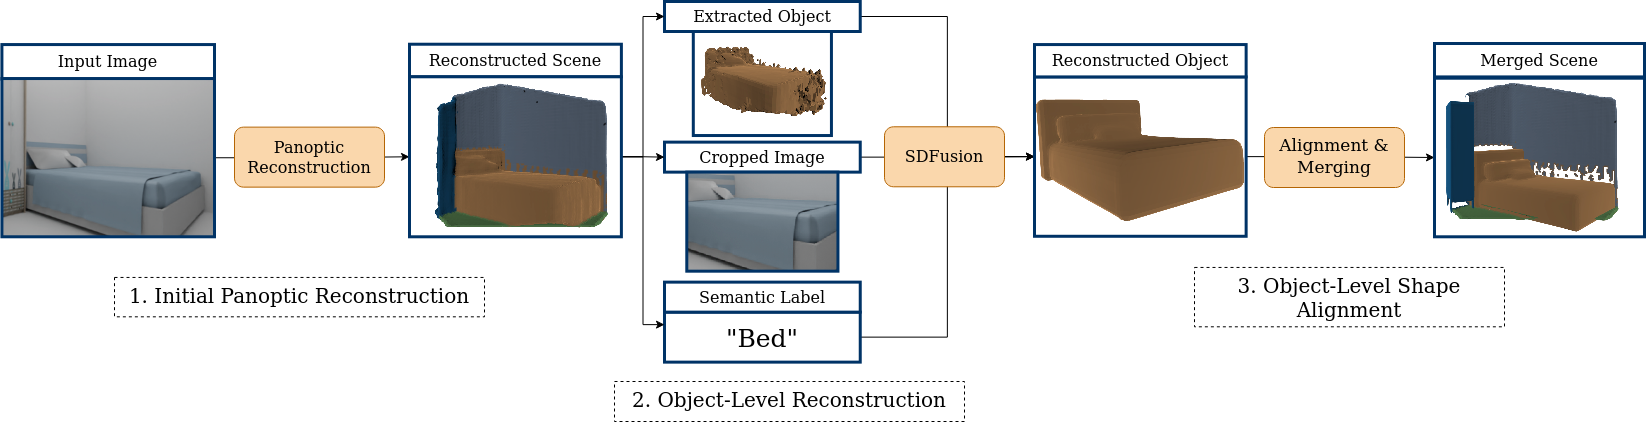
\includegraphics[width=\linewidth]{figs/pipeline.png}
  \caption{The diagram illustrates the multi-step process of panoptic scene reconstruction, object-level reconstruction, and object-level shape alignment. This includes leveraging Panoptic 3D \citep{dahnert2021panoptic} for initial scene reconstruction, SDFusion \citep{cheng2023sdfusion}  for object shape reconstruction, and a custom registration algorithm for precise alignment of reconstructed objects within the scene.}
  \label{fig:pipeline}
\end{figure*}

\subsection{Initial Panoptic Scene Reconstruction}

We leverage Panoptic 3D \citep{dahnert2021panoptic} to predict the camera frustum geometry $\mathbf{X}_{P_{\text{geom}}}$ as well as associated 3D
semantic and instance labels $\mathbf{X}_{P_{\text{sem}}}$, $\mathbf{X}_{P_{\text{instance}}}$  within the image. Said model yields both 2D and 3D representations of detected objects and
does so by employing a ResNet-18 \citep{he2016deep} encoder for feature extraction from the input image. Subsequently,
both a depth encoder and a Mask R-CNN \citep{he2017mask} are applied to the ResNet-18 encoder features to predict both a 2D depth map
and a 2D instance mask.
During training, we learn the 2D output utilizing proxy losses for both depth estimation ($L_d$) and instance segmentation ($L_i$).

% TODO (f.srambical): I don't get this paragraph; also, it does not seem to be complete
%The model is trained to predict geometry, semantic labels, and instance identities for
%sparse voxels within the truncation region. For the geometric loss $L^h_g$ , each hierarchy level is trained
%to predict geometry occupancy using a binary cross entropy loss, and the final hierarchy level also

The depth map facilitates the backprojection of features into a sparse volumetric grid, while the 2D instance mask is propagated to serve as a seed for the 3D instance mask prediction. Finally, a 3D U-Net \citep{cciccek20163d} processes the sparse backprojection to forecast occupancy, distance field, and both semantic and instance labels for each individual occupancy within the grid.

In addition to the proxy losses, binary cross-entropy is used on the occupancy prediction at different hierarchy levels and an $l_1$ loss is employed on the distance field at the final hierarchy level.
The total loss can be formalized as 
\begin{equation}
    \mathcal{L} = w_d \mathcal{L}_d + w_i \mathcal{L}_i + \sum_h (w_g \mathcal{L}_g^h + w_s \mathcal{L}_s^h + w_o \mathcal{L}_o^h),
\end{equation}

where $\mathcal{L}_g^h, \mathcal{L}_s^h, \mathcal{L}_o^h$ represent the geometry as well as 3D semantic and instance label losses at different hierarchy levels, and $w_{x\in\{d, i, g, s, o\}}$ being weighting factors.

At inference time, we use the 2D instance mask to extract RGB crops $\mathbf{I}_{\text{crop}}$ of the input image, and the 3D instance mask to extract the corresponding 3D geometry $\textbf{X}_{P_{\text{geom, crop}}}$.
The extracted image, geometry and the semantic label are subsequently input into the object-level reconstruction model for shape reconstruction.

\subsection{Object-Level Reconstruction}

We use SDFusion \citep{cheng2023sdfusion} for object shape reconstruction, which expects a signed distance field as its primary input, and additionally leverages an RGB image and a textual representation as conditional inputs to guide the reconstruction process. To this end, SDFusion employs task-specific encoders (\citep{radford2021learning, devlin2018bert}) to get image and text embeddings, while simultaneously embedding the 3D shape into a latent space using a pre-trained vector quantized variational autoencoder (VQ-VAE) \citep{oord2017neural}. At training time, noise is introduced to the shape latent via forward diffusion, which is followed by a concatenation of the conditional embeddings. This serves as input to the 3D U-Net \citep{cciccek20163d} denoising network which reconstructs the latent code. Within the denoising U-Net, cross-attention is applied along the concatenated latent code to modulate the denoising process. Ultimately, the VQ-VAE decoder reconstructs the shape.

At inference time, we use SDFusion to output a refined object geometry $\mathbf{X}_S$ for every object-level geometry extraction $\mathbf{X}_{P_{\text{geom, crop}}}$, leveraging the image crop $\mathbf{I}_{\text{crop}}$ and the corresponding semantic label $\mathbf{X}_{P_{\text{sem}}}$.

\subsection{Object-Level Shape Alignment}
The inference output of SDFusion is front-facing and might not align with the object's orientation in the original 3D scene. Thus, to adequately replace the original objects with the refined ones, we employ a custom registration algorithm to ensure proper alignment of the reconstructed objects within the scene. This process consists of 3 key steps:
\begin{enumerate}
    \item \textbf{Position alignment:} To establish a common frame of reference and facilitate subsequent re-orientation, we align the centroid of the refined object with the original object. 
    
    \item \textbf{Rotation \& scale optimization:} Following position alignment, we want to find the correct orientation of our object. As we assume that the object is parallel to the floor and with the right side up, we only iterate through rotations around the y-axis. After each rotation step we scale our refined object in all three directions to fit the initial dimensions. We find the best rotation and scale by sampling points uniformly from both meshes and computing the chamfer distance.  
    
    % TODO (f.srambical): This is vague; what is the distance measure employed? Is it Chamfer distance? Between what? The original and the refined object?
    \item \textbf{Floor alignment:} As most of the instances are standing on the floor, we align the floor distance of our refined object with the lowest vertex of the initial object. This is necessary as the centroids might not have the same object-relative height due to differing geometries. 
\end{enumerate}
Unlike a general approach like ICP, our customized approach leverages domain-specific knowledge about reconstructed indoor scenes in order to limit the degrees of freedom, like rotation in a single direction. This leads to a more robust approach, especially if the geometries are not identical.  